\chapter{Arquitectura}
\label{chap:arquitectura}

\drop{E}{ste} capítulo pretende ofrecer una visión completa de la composición del sistema informático que constituye BreakBrain, profundizando en los diferentes componentes que lo forman y haciendo hincapié en los patrones de diseño utilizados y otros detalles de interés para el lector con conocimientos técnicos.

A lo largo de las siguientes secciones, se presentará la arquitectura detallada del sistema completo, para después estudiar a más bajo nivel los componentes principales por separado, centrando la atención en el del desarrollo de software.

\section{Composición del sistema}

\begin{figure}[h]
  \begin{center}
    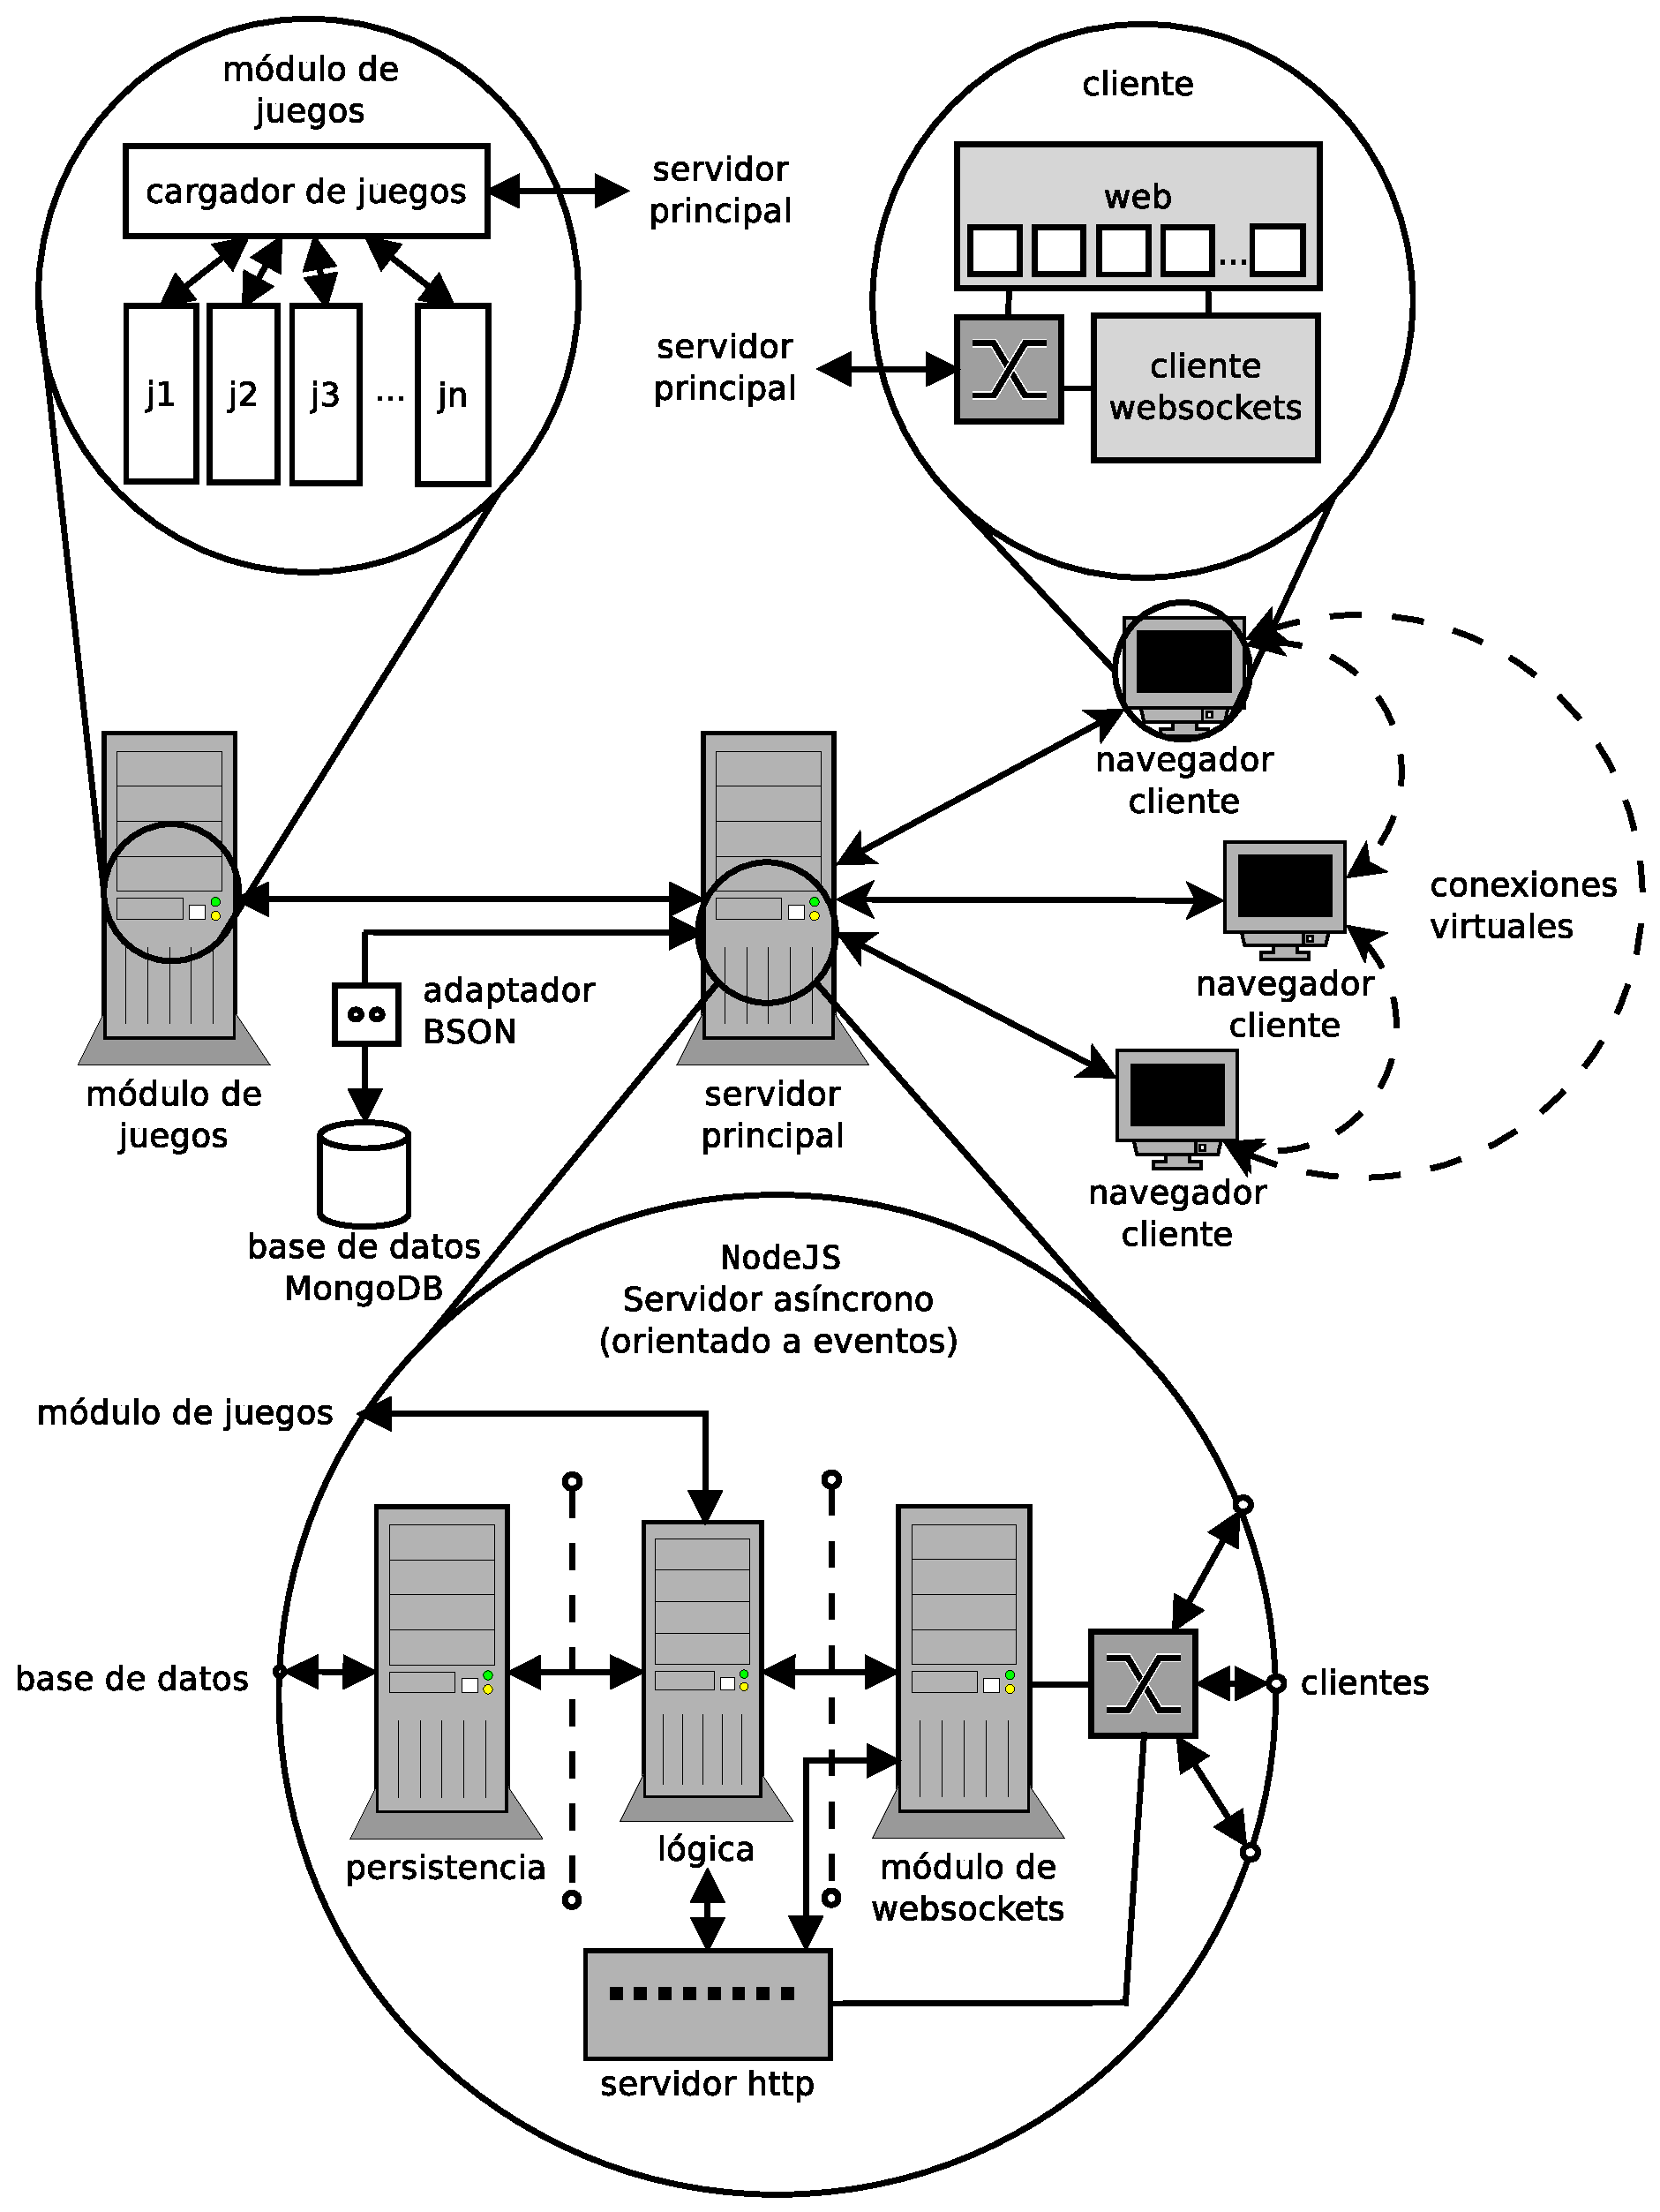
\includegraphics[width=\textwidth]{images/arquitectura.eps}
    \caption{Arquitectura detallada del sistema}
    \label{fig::arquitectura}
  \end{center}
\end{figure}

En la figura \ref{fig::arquitectura} se ofrece una visión detallada del los componentes que forman BreakBrain. Se trata de un enfoque de medio nivel que se adentra en la composición de los diferentes elementos de despliegue del sistema vistos en la sección \ref{sec::despliegue}. Como puede apreciarse, los dos protagonistas del enfoque {\it cliente-servidor} que sigue BreakBrain son tan complejos que se hace patente la necesidad de estudiarlos de forma detallada por separado.

A la vista de la figura \ref{fig::arquitectura} se perciben cuatro elementos esenciales en la composición del sistema:

\begin{itemize}
\item {\bf Cliente}\\Sitio web ejecutado sobre un navegador corriente. El uso de JavaScript que hace BreakBrain es intenso, tanto por la ejecución de los juegos como por el subsistema de comunicación permanente (necesario para los juegos multijugador), por lo que un navegador con buen soporte de JavaScript (como Chrome/Chromium \cite{chrome}) otorgará siempre una mejor experiencia de usuario.
\item {\bf Servidor principal}\\Se trata del corazón del sistema, compuesto principalmente por un servidor web corriente, al que se le ha añaido un servidor de comunicaciones mediante sockets TCP (con mensajes encapsulados en HTTP) para mantener una comunicación ininterrumpida con los clientes, y ofrecer así la base para la ejecución de juegos multijugador. El servidor se ejecuta en Nodester \cite{Nodester}, \acf{PAAS} de Software Libre que ofrece un buen servicio de forma totalmente gratuita.
\item {\bf Servidor de juegos}\\La piedra angular del servicio de juegos monojugador y multijugador. Construido de forma extensible, permite la integración de juegos de terceros en la plataforma. 
\item {\bf Sistema gestor de base de datos}\\Se ha optado por una base de datos no relacional MongoDB, alojada en los servicios de Amazon WS \cite{Amazon} y gestionada por MongoLab \cite{Mongolab}. Este último \acf{SAAS} se encarga del mantenimiento de la base de datos, asegurando un alta disponibilidad y escalabilidad.
\end{itemize}

\section{Arquitectura del sitio web}

\subsection{Patrón MVC}

\section{Arquitectura del servidor}

\subsection{Patrón MVC}

\subsection{Diseño modular}

\subsection{Arquitectura del servidor de juegos}

\section{Sistema Gestor de Base de Datos}



